\documentclass[10pt, a4paper]{article}
\usepackage[top=80pt, bottom=50pt, left=72pt, right=55pt]{geometry}
\usepackage{enumerate}
\usepackage[fleqn]{amsmath}
\usepackage{graphicx}
\begin{document}
\title{PH-105 QM Sheet 2}
\date{23.10.2012}
\author{Vipul Singh}
\maketitle
\begin{enumerate}
\item[71.]{\bf A beam of particles of energy E and de-Broglie wavelength $\lambda$, travelling along the positive x-axis in potential free region, encounters a one-dimensional potential barrier of height $V_{0}$=E and width L.\\
(a) Obtain an expression for the transmission coefficient.\\
(b) For what value of L (in terms of $\lambda$), will the reflection coefficient be half?}\\

{\underline {\bf Solution}} : \\
\begin{center}
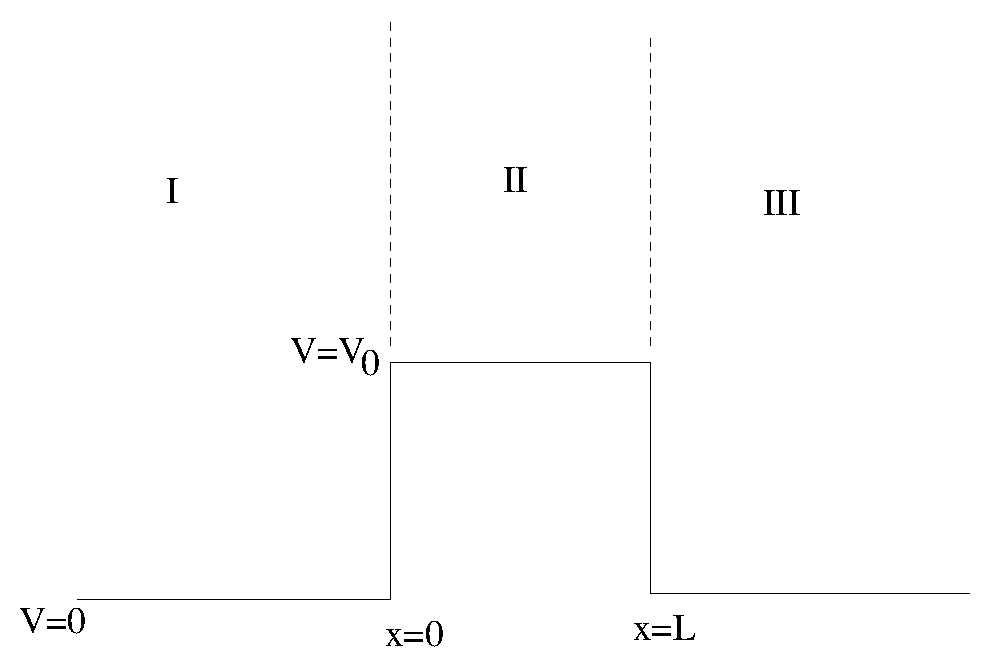
\includegraphics[scale=0.6]{q71.eps}
\end{center}
Let $k^{2}=\frac{2mV_{0}}{\hbar^{2}}$.
Then, the wave-functions in the three regions are given by:\\
$\phi_{I}(x)=Ae^{ikx}+Be^{-ikx}$\\
$\phi_{II}(x)=Cx+D$\\
$\phi_{III}(x)=Fe^{ikx}$\\
At x=0, we have $A+B=D$ and $ik(A-B)=C$. At x=L, we have $CL+D=Fe^{ikL}$ and $C=ikFe^{ikL}$.\\
On solving, we get $\frac{F}{A}=\frac{2e^{-ikL}}{2-ikL}$\\
Transmission coefficient, $T=|\frac{F}{A}|^{2}=\frac{4}{4+(kL)^{2}}$.\\
For $T=0.5$, we get $kL=2$ and hence $L=\frac{2}{k}=\frac{\lambda}{\pi}$.
\end{enumerate}
\end{document}
